\section{Grundlagen}
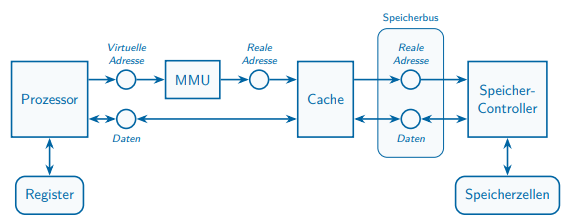
\includegraphics[width = \columnwidth]{grafiken/computer_grundaufbau.png}
Prozessor: automatische Maschine mit internem Zustand (Register) und Schnittstelle für externe Adressen und Daten, fordert selbständig Instruktionen/Daten an und führt diese aus, interne \& externe Zustand kann sich dabei ändern 

\subsection{Prozessor-Zyklus}
1. Prozessor fordert Wert von der Adresse an, die im Befehlszeiger steht.
2. Prozessor decodiert Instruktion aus Wert.
3. Prozessor wählt den zur Instruktion gehörenden Baustein aus.
4. Aktiver Baustein decodiert Parameter aus Wert.
5. Aktiver Baustein liest aus den Registern.
6. Aktiver Baustein führt Berechnung aus.
7. Aktiver Baustein schreibt in die Register.
8. Prozessor erhöht Befehlszeiger entsprechend der Länge der Instruktion.

\subsection{Binärrechnen}
n = Anzahl Stellen

\subsubsection{Minima/Maxima}
\textbf{unsigned/ohne Vorzeichen}: $0...2^{n}-1$\\
\textbf{signed/mit Vorzeichen}:\\
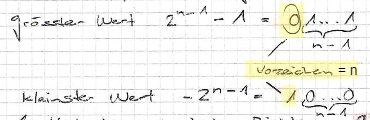
\includegraphics[scale = .75]{grafiken/zweierkomplement1.PNG}
\subsubsection{Zweierkomplement}
Allgemein bei -1 alle Bits gesetzt: 1..1\\
Maximum $2^{n-1}-1$ invertiert = 10..01\\
$N(0) = 0$, $2^{n-1} = N(2^{n-1}) = 100..$

\subsubsection{Invertieren}
\textcolor{yellow}{bestimmt Vorzeichen, 0 = +, 1 = -, index = n}
- 1, invertieren\\
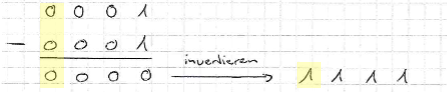
\includegraphics[scale = .5]{grafiken/zweierkomplement3.PNG}